\documentclass[dvipdfmx,11pt]{beamer}

%\usepackage{bxdpx-beamer}
\usepackage{listings,jlisting}
%\usepackage{plistings}
\usepackage{graphicx,xcolor} %文字の色
\usepackage[deluxe]{otf}
\usepackage{txfonts}


\usetheme{Warsaw}

\newcommand{\code}[1]{\lstinline[basicstyle=\ttfamily]{#1}}
\renewcommand{\kanjifamilydefault}{\gtdefault}
\renewcommand{\bibname}{参考文献}
\setbeamersize{text margin left=1.5em,text margin right=1.5em} %文字間の余白調整
\setbeamertemplate{navigation symbols}{} %アイコン消去
\setbeamertemplate{footline}[frame number] %フレーム番号表示
\useoutertheme{shadow}
\usefonttheme{professionalfonts} %数式文字のLaTeX化


\title{解集合プログラミングを用いたグラフ彩色問題の解法に関する考察}
\author{101830314 春田 穂高}
\institute{番原研究室}
\date{2021年度 卒業研究発表会\\2022年2月18日}

\begin{document}
%%%%%%%%%%%%%%%%%%%%%%%%%%%%%%%%%%%%%%%%%%%%%%%%%%%%%%%%%%%%%%%%%%%
\frame{\maketitle}
% %%%%%%%%%%%%%%%%%%%%%%%%%%%%%%%%%%%%%%%%%%%%%%%%%%%%%%%%%%%%%%%%%%%
% \begin{frame}{グラフ彩色問題と関連問題}
%  \begin{itemize}
%   \item \alert{グラフ彩色問題}
%         \begin{itemize}
% 	 \item 与えられた有限無向グラフ$G$の隣接する頂点が
% 	       同色にならないように各頂点を塗りわけるときに,
% 	       必要となる最小の色数を求める問題.
% 	 \item 最適化コンパイラのレジスタ割り付けや
% 	       無線の周波数割り当て等の応用がある.
%         \end{itemize}
%   \item \alert{グラフ彩色判定問題}
%         \begin{itemize}
%          \item 自然数$k\geq 3$について,
% 	       グラフ$G$が$k$色以下で彩色可能かどうかを決定する問題.
%         \end{itemize}
%  \end{itemize}

%  \begin{alertblock}{}
%   \centering
%   グラフ彩色問題はNP困難,グラフ彩色判定問題はNP完全である.
%  \end{alertblock}
% \end{frame}

% %%%%%%%%%%%%%%%%%%%%%%%%%%%%%%%%%%%%%%%%%%%%%%%%%%%%%%%%%%%%%%%%%%%
\begin{frame}{グラフ彩色問題と関連問題}
  \begin{block}{グラフ彩色判定問題}\centering
    与えられた有限無向グラフ$G$と色数$k\geq 3$に対して,
    隣接する頂点が同色にならないように$G$を$k$色以下で彩色可能かど
    うかを決定する問題
    \begin{itemize}
    \item 代表的な組合せ問題で,NP完全であることが知られている.
    \item 最適化コンパイラのレジスタ割り付けや無線の周波数割り当て等の応用がある.
    \end{itemize}
  \end{block}
  \pause
  \begin{alertblock}{本研究が対象とするグラフ彩色最適化問題}
    \begin{itemize}
    \item \textbf{同色頂点数最小化(最大化)問題}
      \begin{itemize}
      \item グラフ彩色判定問題の実行可能解のうち,同色(例えば,赤色)で
        塗られる頂点数の最小値(最大値)を求める問題
      \end{itemize}
    \item \textbf{多色頂点数最大化問題}
      \begin{itemize}
      \item グラフ彩色判定問題の制約を満たしつつ,
        多色(2色以上)で塗られる頂点数の最大値を求める問題である.
      \item この問題の最適解は,基のグラフ彩色判定問題の複数の実行可能解に
        対応し,\alert{\bf 基の問題の圧縮解}とみなすことができる.
      \end{itemize}
    \end{itemize}
  \end{alertblock}
 % \begin{alertblock}{}
 %  \centering
 %  本研究では,グラフ彩色に関する最適化問題を対象とする.%%% あってますか?
 % \end{alertblock}
\end{frame}

%%%%%%%%%%%%%%%%%%%%%%%%%%%%%%%%%%%%%%%%%%%%%%%%%%%%%%%%%%%%%%%%%%%
\begin{frame}{多色頂点数最大化問題の例 [Knuth TAOCP '15]}
  \begin{block}{}\centering
    5次の \code{McGregor}グラフに対する最適解の一例を示す.
  \end{block}

  \begin{tabular}{cc}
  \begin{minipage}[t]{0.5\linewidth}
   \centering
   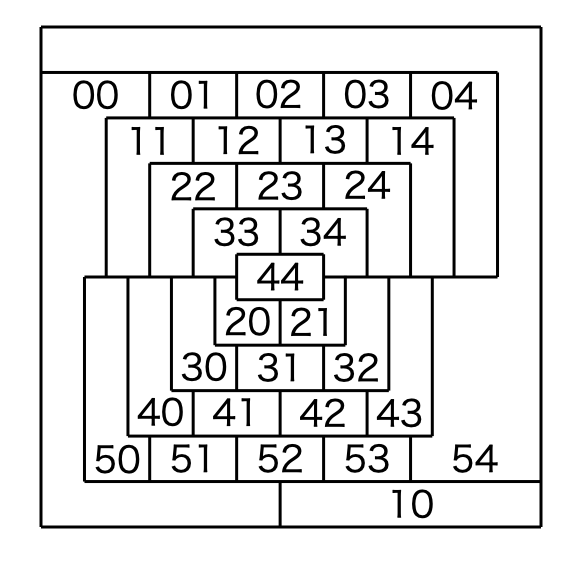
\includegraphics[scale=0.2]{fig/order5.png}
  \end{minipage}
  \begin{minipage}[t]{0.5\linewidth}
   \centering
   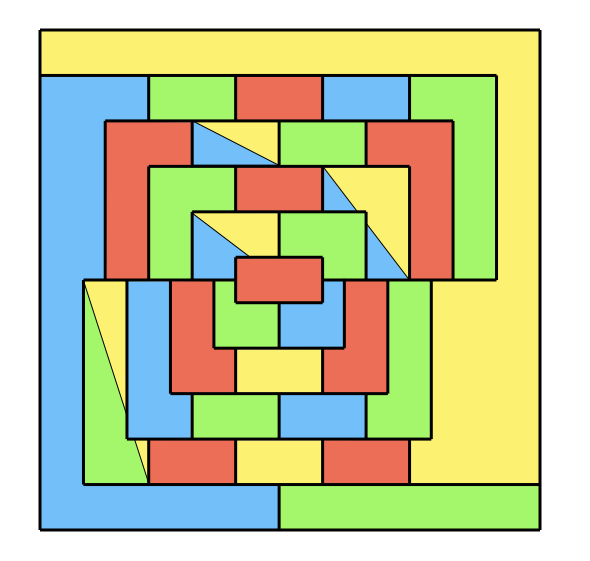
\includegraphics[scale=0.2]{fig/order5_mult.png}
  \end{minipage}
 \end{tabular}

 \begin{itemize}
 \item グラフの各区画が頂点に,区画の隣接関係が辺に対応する.
 \item 次数に関わらず,4色で彩色可能であることが知られている.
 \item 最適値は4で,
   頂点番号\code{12}, \code{24}, \code{33}, \code{50}
   が2色で彩色されている.
 \item この最適解は,基のグラフ彩色判定問題における
   \alert{\bf 16個の実行可能解の圧縮解}とみなすことができる.
 \end{itemize}
\end{frame}
%%%%%%%%%%%%%%%%%%%%%%%%%%%%%%%%%%%%%%%%%%%%%%%%%%%%%%%%%%%%%%%%%%%
\begin{frame}{解集合プログラミング(Answer Set Programming; ASP)}
 \begin{itemize}
  \item \alert{ASP}は,論理プログラミングから派生した
        比較的新しいプログラミングパラダイムである.
  \item \alert{ASP言語}は,一階論理に基づいた知識表現言語の一種である.
  \item \alert{ASPシステム}は,論理プログラムから
        安定モデル意味論~{\scriptsize[Gelfond and Lifschitz, '88]}
        に基づく解集合を計算するシステムである.
  \item 近年,SAT技術を利用する高速なASPシステムが開発され,
        様々な分野への実用的な応用が急速に拡大している.
 \end{itemize}
 
 \begin{alertblock}{グラフ彩色判定問題に対してASPを用いる利点}
  \begin{itemize}
   \item ASP言語の高い表現力により,記号制約を簡潔に記述可能.
   \item 充足不能コアを用いた最適化探索が可能.
%   \item 高速ASPシステムを用いた高速な解探索,解列挙が可能.
  \end{itemize}
 \end{alertblock}
\end{frame}

%%%%%%%%%%%%%%%%%%%%%%%%%%%%%%%%%%%%%%%%%%%%%%%%%%%%%%%%%%%%%%%%%%%
\begin{frame}{研究目的と内容}
 \begin{alertblock}{研究目的}\centering
   ASP 技術を活用して,グラフ彩色最適化問題を効率良く解くソルバーの実
   現を目指す.
 \end{alertblock}

 \begin{block}{研究内容}
  \begin{enumerate}
   \item \structure{3つのグラフ彩色最適化問題を解くASP符号化を考案}
     \begin{itemize}
     \item 同色頂点数最小化問題
     \item 同色頂点数最大化問題
     \item 多色頂点数最大化問題
     \end{itemize}
   \item \structure{\code{McGregor}グラフをベンチマークとした評価実験}
     \begin{itemize}
     \item Knuth の教科書に記載されていない最適値を生成することができた.
     \item 充足不能コアを用いた最適化探索の有効性が確認できた.
     \end{itemize}
   \item \structure{多色頂点数最大化問題に関する考察}
     \begin{itemize}
     \item 12次の\code{McGregor}グラフの最適解が,基のグラフ彩色判定問
       題の\alert{\bf 約680億}もの実行可能解を表していることがわかった.
     \end{itemize}
   \end{enumerate}
 \end{block}
\end{frame}

%%%%%%%%%%%%%%%%%%%%%%%%%%%%%%%%%%%%%%%%%%%%%%%%%%%%%%%%%%%%%%%%%%%
\begin{frame}{多色頂点数最大化問題のASP符号化 (考案)}

\begin{exampleblock}{}
 \lstinputlisting[frame=none,numbers=left,basicstyle=\ttfamily]{code/color_mult.lp}
\end{exampleblock}

 \begin{itemize}
  \item \code{c(1..k)}は色を表すアトム\code{c(1)},\ldots,\code{c(k)}の略記である.
        %1行目のkは彩色に使用できる色数を定義している.
  \item 2行目は,各頂点\code{X}が各色\code{C}で彩色されることを意味するアトム\code{color(X,C)}を導入し,
        真になる個数を1以上に強制している.
        %1つ以上の色で彩色されることを意味している.
  \item 3行目は,各辺\code{(X,Y)}に対して,頂点\code{X}と頂点\code{Y}が同じ色\code{C}で彩色されないことを表している.
        %隣接する頂点は同色で彩色されないことを意味している.
  \item 5--6行目では,頂点\code{X}が2色以上で彩色されることを意味する補助アトム\code{mult(X)}を導入し,
        その数を最大化している.


  % \item 5行目では2色以上で彩色される頂点が存在している場合,新たなアトム(mult(X))を作成している.
  % \item 6行目では5行目で作成したアトムの数を最大化している.
 \end{itemize}

\end{frame}
%%%%%%%%%%%%%%%%%%%%%%%%%%%%%%%%%%%%%%%%%%%%%%%%%%%%%%%%%%%%%%%%%%%

% %%%%%%%%%%%%%%%%%%%%%%%%%%%%%%%%%%%%%%%%%%%%%%%%%%%%%%%%%%%%%%%%%%%
% \begin{frame}{多色頂点数最大化問題のASP符号化 (提案)}
% TODOTODOTODOTODOTODOTODOTODOTODOTODOTODO

%   \begin{block}{グラフ彩色判定問題の表現}
%   与えられた有限無向グラフ$G$と自然数$k\geq 3$について,
%   以下2つの制約を満たすように$G$の各頂点を
%   $k$色以下で彩色可能かを決定する問題.
%   \begin{itemize}
%    \item $G$の各頂点は一つの色で彩色される.(彩色制約)
%    \item $G$の隣接する頂点は同色で彩色されない.(隣接制約)
%   \end{itemize}
%  \end{block}
%  \begin{enumerate}
%    \item \structure{color符号化}:
%          \begin{itemize}
%           \item グラフ彩色判定問題の彩色制約と隣接制約を簡潔に表現した.
%          \end{itemize}
%   \item \alert{minimize符号化}:%%% 同色頂点数最小化問題と記述したい
%         \begin{itemize}
%          \item color符号化をベースに,
%                ASPの最小化関数~\texttt{\#minimize} を用いて,
% 	       同色で塗られる頂点数を最小化する目的関数を追加.
%         \end{itemize}
%   \item \alert{maximize符号化}:%%% 同色頂点数最大化問題と記述したい
%         \begin{itemize}
%          \item color符号化をベースに,
%                ASPの最大化関数~\texttt{\#maximize} を用いて,
% 	       同色で塗られる頂点数を最大化する目的関数を追加.
%         \end{itemize}
%   \item \alert{mult符号化}:%%% 多色頂点数最大化問題と記述したい
%         \begin{itemize}
%          \item color符号化をベースに,
% 	       1つの頂点を多色で彩色できるように彩色制約の上限を緩和.
%          \item ASPの最大化関数~\texttt{\#maximize} を用いて,
% 	       多色で彩色できる頂点数を最大化する目的関数を追加.
%         \end{itemize}
%  \end{enumerate}
% \end{frame}

%%%%%%%%%%%%%%%%%%%%%%%%%%%%%%%%%%%%%%%%%%%%%%%%%%%%%%%%%%%%%%%%%%%
% \begin{frame}{実験概要}
%  \begin{block}{}
%   考案した符号化の有効性を評価するために各問題の実験を行った.
%  \end{block}

% \begin{itemize}
%  \item \structure{ベンチマーク問題}: order~3$\sim$140のMcGregorグラフ(計138問)
%  \item \structure{ASPシステム}: \textit{clingo}-5.5.0
%  \item \structure{実験環境}: Mac mini Intel Core i7 3.2GHz 64GBメモリ
%  \item \structure{制限時間}: 
%        \begin{itemize}%%% 問題に対してでなくて良いか
%         \item color符号化: 30分
%         \item minimize,maximize,mult符号化: 1時間
%        \end{itemize}
% \end{itemize}  

%  \begin{alertblock}{color符号化の実験結果}
%   order~3$\sim$138の計136問について4彩色可能であると判定できた.
%  \end{alertblock}
 
% \end{frame}

%%%%%%%%%%%%%%%%%%%%%%%%%%%%%%%%%%%%%%%%%%%%%%%%%%%%%%%%%%%%%%%%%%%
\begin{frame}{実験概要}
 \begin{block}{}\centering
   考案した符号化の有効性を評価するために各問題の実験を行った.
 \end{block}
 \vfill
 \begin{itemize}
 \item \structure{ベンチマーク問題}: $N$次の\code{McGregor}グラフ
   \begin{itemize}
   \item 同色頂点数最小化問題: $3 \leq N\leq 20$
   \item 同色頂点数最大化問題: $3 \leq N\leq 38$
   \item 多色頂点数最大化問題: $3 \leq N\leq 15$
   \end{itemize}
 % \item \structure{使用したASP符号化 (提案)}
 %   \begin{itemize}
 %   \item 同色頂点数最小化問題のASP符号化
 %   \item 同色頂点数最大化問題のASP符号化
 %   \item 多色頂点数最大化問題のASP符号化
 %   \end{itemize}
 \item \structure{ASPシステム}: \textit{clingo}-5.5.0
 \item \structure{最適値探索の戦略}: 分枝限定法(BB)と充足不能コア(USC)
 \item \structure{制限時間}: 1時間/問
 \item \structure{実験環境}: Mac mini Intel Core i7 3.2GHz 64GBメモリ  
 \end{itemize}
\end{frame}
%%%%%%%%%%%%%%%%%%%%%%%%%%%%%%%%%%%%%%%%%%%%%%%%%%%%%%%%%%%%%%%%%%%
\begin{frame}{多色頂点数最大化問題の実験結果(最適値と最良値)}
 % \begin{block}{}
 %  \structure{問題}: $N$次の\code{McGregor}グラフ ($3 \leq N\leq 15$: 計13問)
 % \end{block}
 
 \begin{center}
     \tabcolsep = 5mm
     \renewcommand{\arraystretch}{0.9}
     \begin{tabular}{r|r|r}
 %n& h(n)\\
 N&BB &USC\\
 \hline
 3&1*&1*\\
 4&3*&3*\\
 5&4*&4*\\
 6&7*&7*\\
 7&9*&9*\\
 8&13*&13*\\
 9&18*&18*\\
 10&23&\textbf{23*}\\
 11&27&\textbf{\textcolor{red}{29*}}\\
 12&34&\textbf{\textcolor{red}{36*}}\\
 13&\textbf{39}&15\\
 14&\textbf{44}&11\\
 15&\textbf{49}&20\\\hline
\end{tabular}


 \end{center}

 \begin{itemize}
 \item BB法では7問,USC法では10問の最適値を求めることができた.
 \item $N = 11,12$ の2問について,Knuth の教科書に未記載の
   最適値を発見することができた.
 \end{itemize}
\end{frame}

%%%%%%%%%%%%%%%%%%%%%%%%%%%%%%%%%%%%%%%%%%%%%%%%%%%%%%%%%%%%%%%%%%%
\begin{frame}{多色頂点数最大化問題の実験結果に関する考察}
  \begin{alertblock}{}\centering
    多色頂点数最大化問題の最適解が,基のグラフ彩色判定問題のいくつの実
    行可能解を表現しているかについて調査した.
  \end{alertblock}
  \vfill
 
  \begin{center}
    \begin{tabular}{r|c|c|c}
 \hline
 n& h(n)& 圧縮された解の個数& 圧縮率 \\
 \hline
 3&	1&	2&	1.3889 \\
 4&	3&	8&	0.3367 \\
 5&	4&	16&	0.0368 \\
 6&	7&	128&	0.0049 \\
 7&	9&	512&	0.0002 \\
 8&	13&	8192&	- \\
 9&	18&	262144&	- \\
 10&	23&	8388608&	- \\
 11&	29&	536870912&	- \\
 12&	36&	68719476736&	- \\
\end{tabular}
\caption{多色頂点数最大化問題の解の圧縮率}
\label{table:com}
  \end{center}

 \begin{itemize}
  % \item 多色頂点数最大化問題で最適値を発見できた
  %       $3 \leq N\leq 12$までの計10問の解の圧縮に成功した.
  \item $N = 12$ では基のグラフ彩色判定問題の
    \alert{\bf 約680億}もの実行可能解を表していることがわかった.
 \end{itemize}
\end{frame}

%%%%%%%%%%%%%%%%%%%%%%%%%%%%%%%%%%%%%%%%%%%%%%%%%%%%%%%%%%%%%%%%%%%
\begin{frame}{まとめと今後の課題}

  \begin{enumerate}
   \item \structure{3つのグラフ彩色最適化問題を解くASP符号化を考案}
     \begin{itemize}
       \item ASPの高い表現力により簡潔に記述できることが確認できた.
     \end{itemize}
   \item \structure{\code{McGregor}グラフをベンチマークとした評価実験}
     \begin{itemize}
     \item 21問について,Knuth の教科書に記載されていない最適値を生成することができた.
     \item 充足不能コアを用いた最適化探索の有効性が確認できた.
     \end{itemize}
   \item \structure{多色頂点数最大化問題に関する考察}
     \begin{itemize}
     \item 12次の\code{McGregor}グラフの最適解が,基のグラフ彩色判定問
       題の\alert{\bf 約680億}もの実行可能解を表していることがわかった.
     \end{itemize}
   \end{enumerate}

   \begin{block}{今後の課題}
     \begin{itemize}
     \item 対称性除去を用いた考案ASP符号化の改良
     \item McGregorグラフ以外のグラフでの評価実験
     \item 多色頂点数最大化問題のASP符号化を応用し,
       様々な組合せ問題の実行可能解の圧縮可能性を調査
     \end{itemize}
   \end{block}
 \end{frame}

%%%%%%%%%%%%%%%%%%%%%%%%%%%%%%%%%%%%%%%%%%%%%%%%%%%%%%%%%%%%%%%%%%%

% \begin{frame}[noframenumbering]{参考文献}
%  \bibliographystyle{jplain} % 参考文献スタイル
%  \bibliography{aisat,bachelor}    % 参考文献リスト
% \end{frame}

%%%%%%%%%%%%%%%%%%%%%%%%%%%%%%%%%%%%%%%%%%%%%%%%%%%%%%%%%%%%%%%%%%%
\appendix
\begin{frame}[noframenumbering]{}
 \thispagestyle{empty}
 \Huge 付録
\end{frame}

%%%%%%%%%%%%%%%%%%%%%%%%%%%%%%%%%%%%%%%%%%%%%%%%%%%%%%%%%%%%%%%%%%%
\begin{frame}[noframenumbering]{ \code{McGregor} グラフ[Knuth2015]}
 \thispagestyle{empty}
 \begin{exampleblock}{5次の \code{McGregor} グラフ}
  \begin{center}
   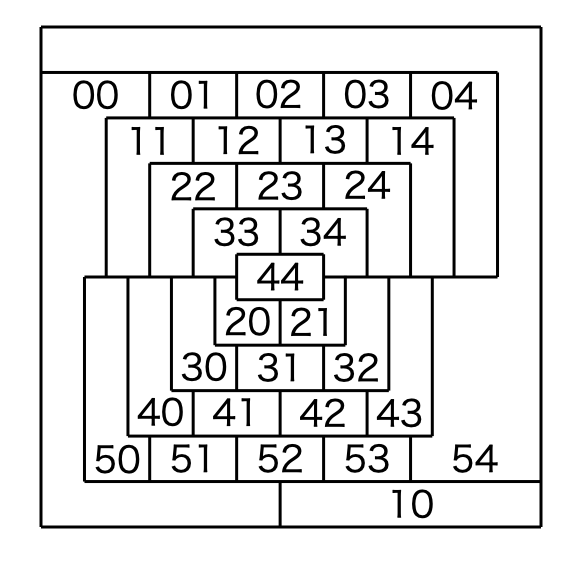
\includegraphics[scale=0.2]{fig/order5.png}
  \end{center}
 \end{exampleblock}

 \begin{itemize}
  % \item D.~E~.Knuthの教科書
  %        The Art of Computer Programming~\cite{Knuth:TAOCP:SAT}
  %        に記載されているグラフである.
  \item \code{McGregor} グラフの各区画が頂点に,区画の隣接関係が辺に対応.
  \item グラフを構成する頂点や辺は次数$n$によって定まり,
	頂点数は$N=n*(n+1)$個,辺数は$3N-6$本である.%\cite{Knuth:TAOCP:SAT}
  \item 次数$n$に関わらず,4色で彩色可能であることが知られている.
 \end{itemize}
\end{frame}
%%%%%%%%%%%%%%%%%%%%%%%%%%%%%%%%%%%%%%%%%%%%%%%%%%%%%%%%%%%%%%%%%%%
\begin{frame}[noframenumbering]{同色頂点数最小化問題の実験結果(最適値と最良値)}
 \thispagestyle{empty}
 \begin{block}{}
  \structure{問題}: $N$次の\code{McGregor}グラフ ($3 \leq N\leq 20$: 計18問)
 \end{block}

 \begin{center}
  \begin{tabular}{r|c|c}
 %n& f(n)\\
 N&BB &USC\\
 \hline
 3&2*&2*\\
 4&2*&2*\\
 5&3*&3*\\
 6&4*&4*\\
 7&5*&5*\\
 8&7*&7*\\
 9&7*&7*\\
 10&7*&7*\\
 11&8*&8*\\
 12&9*&9*\\
 13&10*&10*\\
 14&12&\textbf{12*}\\
 15&\textbf{12}&49\\
 16&16&\textbf{12*}\\
 17&21&\textbf{\textcolor{red}{13*}}\\
 18&19&\textbf{\textcolor{red}{14*}}\\
 19&\textbf{20}&58\\
 20&\textbf{22}&59\\\hline
\end{tabular}


 \end{center}

 \begin{itemize}
  \item BB法が優れていた問題は3問,
        USC法が優れていた問題は4問.
  \item BB法は11問,USC法は15問において,
	最適値を求ていた.
  \item $N = 17,18$ の2問について
	新たに最適値を発見することができた.
 \end{itemize}
\end{frame}

%%%%%%%%%%%%%%%%%%%%%%%%%%%%%%%%%%%%%%%%%%%%%%%%%%%%%%%%%%%%%%%%%%%
\begin{frame}[noframenumbering]{同色頂点数最大化問題の実験結果(最適値と最良値)}
 \thispagestyle{empty}
 \begin{block}{}
  \structure{問題}: $N$次の\code{McGregor}グラフ ($3 \leq N\leq 38$: 計36問)
 \end{block}
 

 \begin{center}
  \begin{table}[tb]\scriptsize
   \begin{table}[t]\scriptsize
%\renewcommand{\arraystrech}{1.2}
\begin{tabular}{r|cc||r|cc||r|cc}
 \hline
 %n& g(n)\\
 N&BB &USC&N&BB&USC&N&BB&USC\\
 \hline
 3&4*&4*&    15&71&\textbf{77*}&
 27&\textbf{185}&180 \\
 4&6*&6*&    16&71&\textbf{88*}&
 28&199&\textbf{\textcolor{red}{266*}} \\
 5&10*&10*&    17&76&\textbf{\textcolor{red}{99*}}&
 29&221&\textbf{\textcolor{red}{285*}} \\
 6&13*&13*&    18&91&\textbf{\textcolor{red}{111*}}&
 30&224&\textbf{\textcolor{red}{305*}} \\
 7&17*&17*&    19&92&\textbf{\textcolor{red}{123*}}&
 31&247&\textbf{\textcolor{red}{325*}} \\
 8&23*&23*&    20&109&\textbf{\textcolor{red}{137*}}&
 32&255&255 \\
 9&28&\textbf{28*}&    21&121&\textbf{\textcolor{red}{150*}}&
 33&\textbf{280}&278 \\
 10&35&\textbf{35*}&    22&122&\textbf{\textcolor{red}{165*}}&
 34&296&\textbf{\textcolor{red}{391*}} \\
 11&42&\textbf{42*}&    23&137&\textbf{\textcolor{red}{180*}}&
 35&310&\textbf{\textcolor{red}{414*}} \\
 12&49&\textbf{50*}&    24&146&\textbf{\textcolor{red}{196*}}&
 36&338&\textbf{\textcolor{red}{438*}} \\
 13&56&\textbf{58*}&    25&162&\textbf{\textcolor{red}{212*}}&
 37&\textbf{348}&340 \\
 14&56&\textbf{68*}&    26&180&\textbf{\textcolor{red}{230*}}&
 38&371&371 \\ 
\end{tabular}
\end{table}

  \end{table}
 \end{center}


 \begin{itemize}
  \item BB法が優れていた問題は3問,
        USC法が優れていた問題は25問.
  \item BB法では6問,USC法が31問において,
	最適値を求めていた.
  \item 17問について,新たに最適値を発見することができた.
 \end{itemize}
\end{frame}
%%%%%%%%%%%%%%%%%%%%%%%%%%%%%%%%%%%%%%%%%%%%%%%%%%%%%%%%%%%%%%%%%%%
\begin{frame}[noframenumbering]{グラフ彩色問題の実行可能解の全解列挙(1/2)}
 \thispagestyle{empty}

 \begin{block}{}
  %グラフ彩色における多色頂点数最大化問題の実行可能解の圧縮を確認するために,
  グラフ彩色問題の実行可能解の全解列挙する実験を行った.  
 \end{block}

 \begin{block}{実験概要}
  \begin{itemize}
   \item \structure{ASPシステム}: \textit{clingo}-5.5.0
   \item \structure{実験環境}: Mac mini Intel Core i7 3.2GHz 64GBメモリ
   \item \structure{制限時間}: 1時間
   \item \structure{問題数}: $N$次の\code{McGregor}グラフ ($3 \leq N\leq 10$: 計8問)
  \end{itemize}
 \end{block}
\end{frame}

%%%%%%%%%%%%%%%%%%%%%%%%%%%%%%%%%%%%%%%%%%%%%%%%%%%%%%%%%%%%%%%%%%%
\begin{frame}[noframenumbering]{グラフ彩色問題の実行可能解の全解列挙(2/2)}
 \thispagestyle{empty}

 \begin{center}
  \begin{tabular}{r|r|r}
 \hline
 N& 解の総数& CPU時間\\
 3&144*&0.002\\
 4&2376*&0.009\\
 5&43536*&0.143\\
 6&2589768*&7.796\\
 7&224442336*&865.500\\
 8&$\geq$816623222&-\\
 9&$\geq$676088853&-\\
 10&$\geq$504392039&-\\
\end{tabular}

 \end{center}

 \begin{itemize}
  \item $3 \leq N\leq 7$までの計5問について全解列挙に成功した.
 \end{itemize}
\end{frame}

%%%%%%%%%%%%%%%%%%%%%%%%%%%%%%%%%%%%%%%%%%%%%%%%%%%%%%%%%%%%%%%%%%%
\end{document}


%%% Local Variables:
%%% mode: japanese-latex
%%% TeX-master: t
%%% End:
